\documentclass[tikz,convert={density=300,outext=.png}]{standalone}
\usetikzlibrary{calc}

\begin{document}
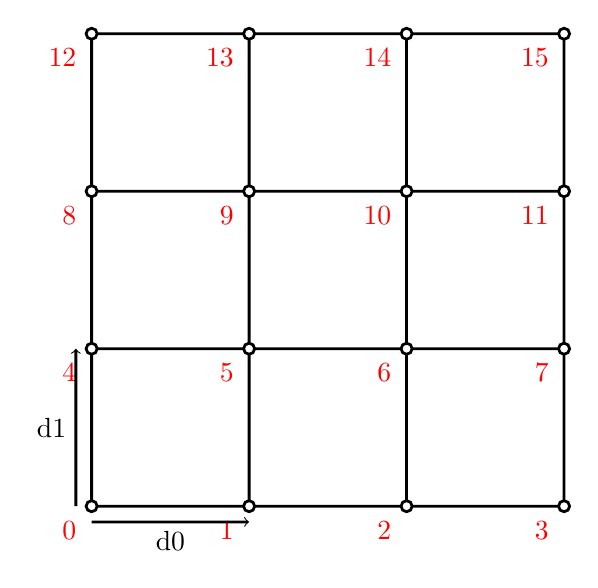
\begin{tikzpicture}[transparency group=knockout]
\coordinate (dx) at (2,0);
\coordinate (dy) at (0,2);
\coordinate (a0) at ($0.866*(dy)-0.5*(dx)$);
\coordinate (a1) at ($(a0)+(dy)$);
\coordinate (a2) at ($(a1)+(dy)$);
\coordinate (a3) at ($(a2)+(dy)$);
\coordinate (b0) at ($(a0)+(dx)$);
\coordinate (b1) at ($(b0)+(dy)$);
\coordinate (b2) at ($(b1)+(dy)$);
\coordinate (b3) at ($(b2)+(dy)$);
\coordinate (c0) at ($(b0)+(dx)$);
\coordinate (c1) at ($(c0)+(dy)$);
\coordinate (c2) at ($(c1)+(dy)$);
\coordinate (c3) at ($(c2)+(dy)$);
\coordinate (d0) at ($(c0)+(dx)$);
\coordinate (d1) at ($(d0)+(dy)$);
\coordinate (d2) at ($(d1)+(dy)$);
\coordinate (d3) at ($(d2)+(dy)$);

\draw (a0) -- (a1) (b0) -- (b1) (c0) -- (c1) (d0) -- (d1) (a1) -- (a2) (b1) -- (b2) (c1) -- (c2) (d1) -- (d2) (a2) -- (a3) (b2) -- (b3) (c2) -- (c3) (d2) -- (d3);
\draw (a0) -- (b0) (a1) -- (b1) (a2) -- (b2) (a3) -- (b3) (b0) -- (c0) (b1) -- (c1) (b2) -- (c2) (b3) -- (c3) (c0) -- (d0) (c1) -- (d1) (c2) -- (d2) (c3) -- (d3);

\node[below left=2pt,fill,opacity=0,text opacity=1,color=red] at (a0) {0};
\node[below left=2pt,fill,opacity=0,text opacity=1,color=red] at (b0) {1};
\node[below left=2pt,fill,opacity=0,text opacity=1,color=red] at (c0) {2};
\node[below left=2pt,fill,opacity=0,text opacity=1,color=red] at (d0) {3};
\node[below left=2pt,fill,opacity=0,text opacity=1,color=red] at (a1) {4};
\node[below left=2pt,fill,opacity=0,text opacity=1,color=red] at (b1) {5};
\node[below left=2pt,fill,opacity=0,text opacity=1,color=red] at (c1) {6};
\node[below left=2pt,fill,opacity=0,text opacity=1,color=red] at (d1) {7};
\node[below left=2pt,fill,opacity=0,text opacity=1,color=red] at (a2) {8};
\node[below left=2pt,fill,opacity=0,text opacity=1,color=red] at (b2) {9};
\node[below left=2pt,fill,opacity=0,text opacity=1,color=red] at (c2) {10};
\node[below left=2pt,fill,opacity=0,text opacity=1,color=red] at (d2) {11};
\node[below left=2pt,fill,opacity=0,text opacity=1,color=red] at (a3) {12};
\node[below left=2pt,fill,opacity=0,text opacity=1,color=red] at (b3) {13};
\node[below left=2pt,fill,opacity=0,text opacity=1,color=red] at (c3) {14};
\node[below left=2pt,fill,opacity=0,text opacity=1,color=red] at (d3) {15};

\draw[fill=white] (a0) circle(2pt); 
\draw[fill=white] (a1) circle(2pt);
\draw[fill=white] (a2) circle(2pt);
\draw[fill=white] (a3) circle(2pt); 
\draw[fill=white] (b0) circle(2pt); 
\draw[fill=white] (b1) circle(2pt); 
\draw[fill=white] (b2) circle(2pt); 
\draw[fill=white] (b3) circle(2pt); 
\draw[fill=white] (c0) circle(2pt); 
\draw[fill=white] (c1) circle(2pt); 
\draw[fill=white] (c2) circle(2pt); 
\draw[fill=white] (c3) circle(2pt);
\draw[fill=white] (d0) circle(2pt);
\draw[fill=white] (d1) circle(2pt); 
\draw[fill=white] (d2) circle(2pt);
\draw[fill=white] (d3) circle(2pt);

\coordinate (d1_0) at ($(a0)-0.1*(dx)$);
\coordinate (d1_1) at ($(a1)-0.1*(dx)$);
\coordinate (d0_0) at ($(a0)-0.1*(dy)$);
\coordinate (d0_1) at ($(b0)-0.1*(dy)$);

\draw [->] (d0_0) -- (d0_1);
\draw [->] (d1_0) -- (d1_1);

\node[below] at ($0.5*(d0_0)+0.5*(d0_1)$) {d0};
\node[left] at ($0.5*(d1_0)+0.5*(d1_1)$) {d1};

\end{tikzpicture}



\end{document}
